\documentclass[a4paper,12pt,oneside,pdflatex,italian,final,twocolumn]{article}

\usepackage[utf8]{inputenc}
\usepackage{parallel}
\usepackage{siunitx}
\usepackage{booktabs}
\usepackage{fancyhdr}
\usepackage[export]{adjustbox}
\usepackage[top=1.0in,bottom=0.8in,left=0.7in,right=0.7in]{geometry}
\usepackage{libertine}
\renewcommand*\familydefault{\sfdefault} 
\usepackage[T1]{fontenc}
\usepackage{amsmath}

\title{PROMETHEUS}
\author{Inbiodroid}
\date{August 2025}

\begin{document}

% --- Cover Page ---
\begin{titlepage}
    \centering
    \vspace*{0.5cm}

    
\includegraphics[width=0.4\textwidth]{logo.png}\par
    \vspace{1cm}

    {\Huge \textbf{PROMETHEUS}}\par
    \vspace{0.5cm}
    {\Large \textbf{v3.0}}\par
    \vspace{0.5cm}

    % Insert additional image here
    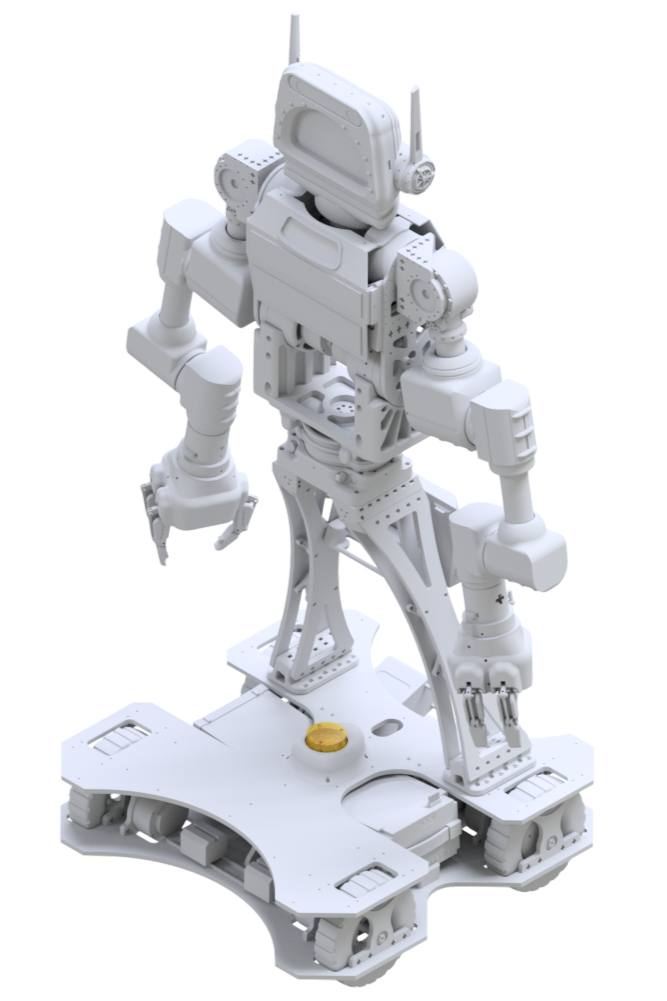
\includegraphics[width=0.5\textwidth]{PR3iso3D.png}\par
    \vspace{0.5cm}

    {\LARGE Inbiodroid}\par
    \vspace{0.5cm}
    {\large Hoja Técnica}\par
    \vfill

    {\large Diciembre de 2025}\par
\end{titlepage}

% --- Start of main content ---
\pagestyle{fancy}
\lhead{Inbiodroid}
\rhead{PROMETHEUS 3.0}
\fancyfoot[C]{\thepage}

\onecolumn

% --- Header Figure ---
\begin{figure}[h!]
\begin{minipage}{0.4\textwidth}
\centering

\includegraphics[width=.8\textwidth,center]{logo.png}
\end{minipage}
\hfill
\begin{minipage}{0.4\textwidth}
\centering
\Huge \textbf{Prometheus 3.0}
\end{minipage}
\end{figure}

% --- Resumen Section ---
\begin{figure}[h!]
\begin{minipage}{0.5\textwidth}
\section{Resumen}
\begin{itemize}
    \item Sistema de Telepresencia Avatar
    \item Robot Teleoperado y Cabina de Operación 
    \item Entorno de Realidad Virtual
    \item Comunicación Inalámbrica (UDP)
    \item +5 horas en Operación
\end{itemize}
\end{minipage}
\hfill
\begin{minipage}{0.65\textwidth}
\centering
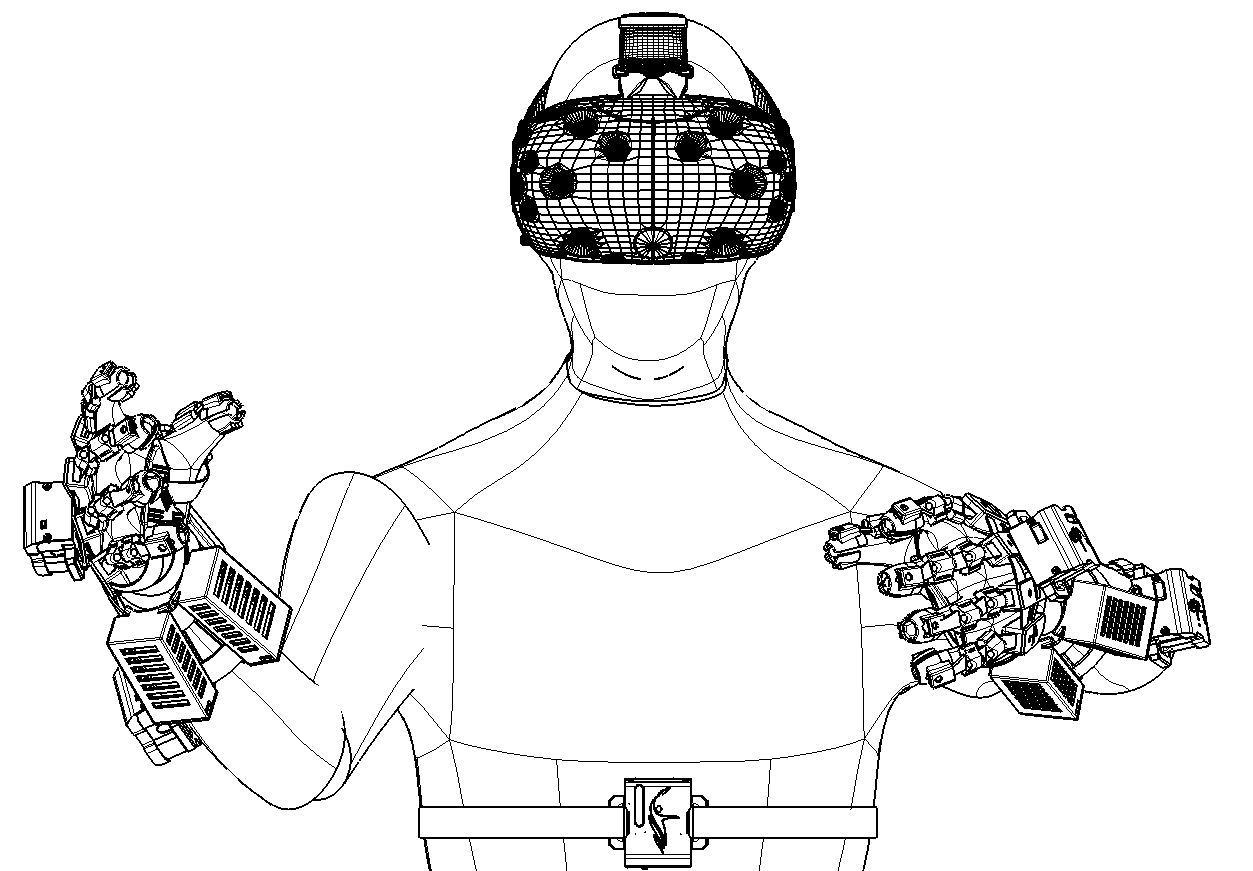
\includegraphics[width=0.8\textwidth,left]{Operador_CloseUp.PNG}
\end{minipage}
\end{figure}

% --- Rest of the document ---
\vspace{-2em}
\section{Descripción General}
\begin{itemize}
\item Sistema de telepresencia robótica humanoide diseñado para extender la presencia física, cognitiva y sensorial de un operador humano en entornos remotos. 
\item Arquitectura dividida en dos secciones funcionales principales:
    \begin{itemize}
    \item Zona de operador: Conjunto de interfaces de percepción y control que capturan los movimientos, gestos y acciones del usuario, y proporcionan retroalimentación sensorial inmersiva para la teleoperación del sistema.
    \item Robot humanoide: Plataforma robótica humanoide modular que reproduce en tiempo real los movimientos del operador, integra sensores de percepción y navegación, y ejecuta acciones físicas en el entorno remoto.
    \end{itemize}
\end{itemize}

\vspace{-1.5em}
\begin{center}
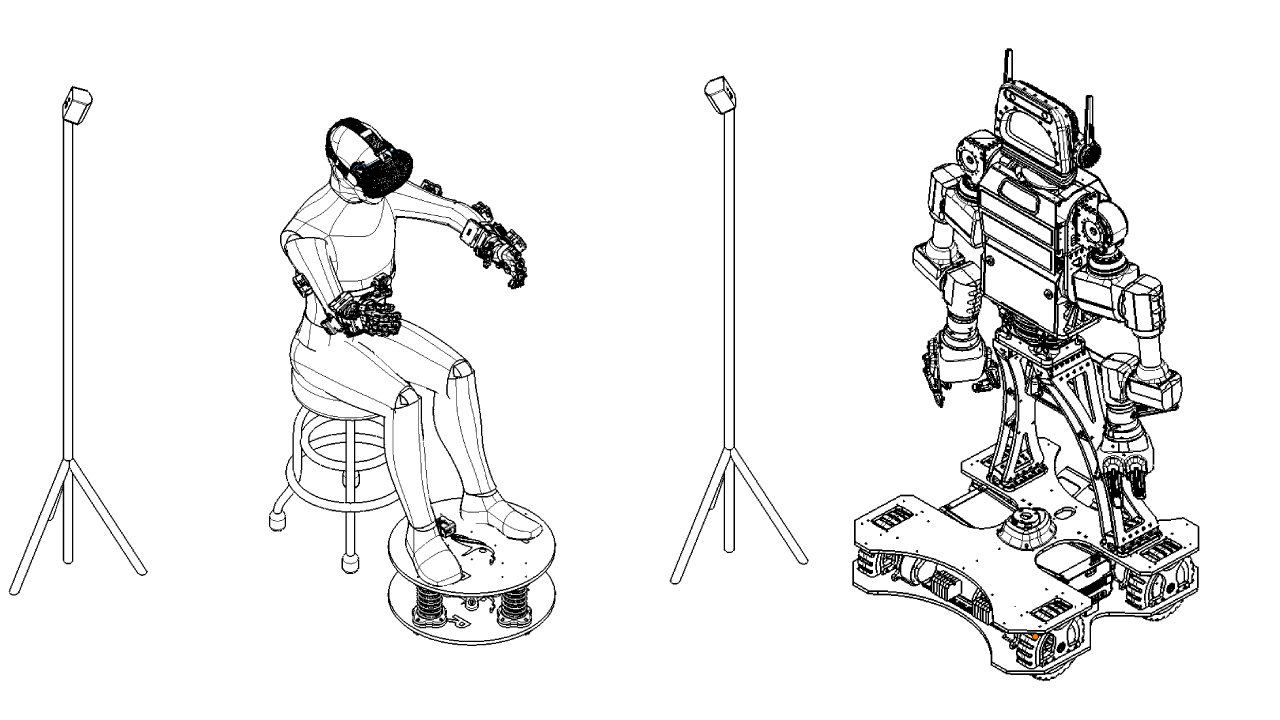
\includegraphics[width=0.9\textwidth]{PR3full.png}
\end{center}
\vspace{-2em}

\section{Características de Funcionamiento}
\begin{itemize}
 \item Zona del Operador:
 \begin{itemize}
    \item Módulos de captura de movimiento de torso y brazos mediante sensores inerciales (IMUs) con retroalimentación vibratoria háptica.
    \item Guantes hápticos para el control preciso de los sujetadores del robot.
 \end{itemize}
\end{itemize}

\begin{figure}[h!]
\begin{minipage}{0.5\textwidth}
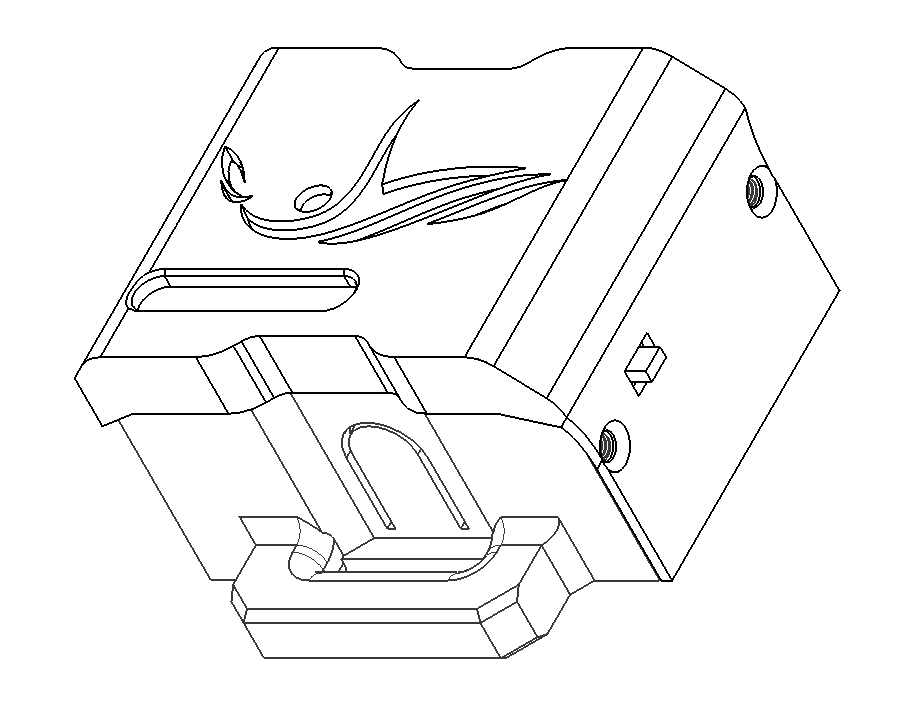
\includegraphics[width=0.6\textwidth,center]{Hermes_Isometrico_2.PNG}
\end{minipage}
\hfill
\begin{minipage}{0.7\textwidth}
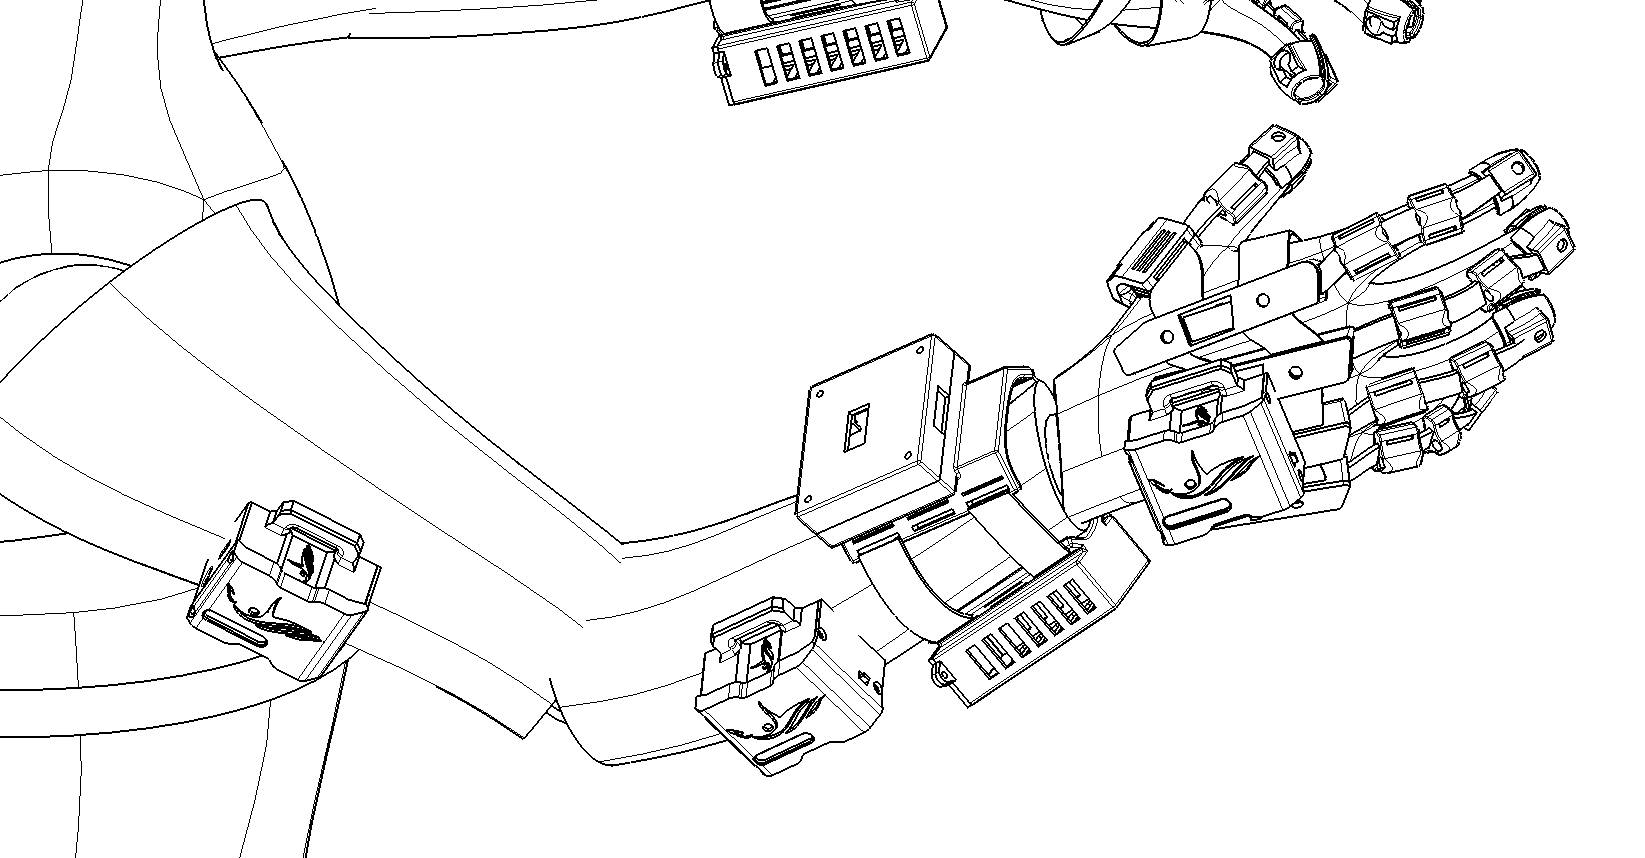
\includegraphics[width=0.7\textwidth,left]{Brazo_CloseUp.PNG}
\end{minipage}
\end{figure}

\vspace{-1em}

\begin{itemize}
    \begin{itemize}
        \item Sistema de dirección plantar que detecta la inclinación de los pies para controlar la locomoción del humanoide.
        \item Visor de realidad virtual HTC Pro Eye para visualización estereoscópica del entorno remoto, detección de movimientos de cabeza y transmisión de audio binaural.
    \end{itemize}
\end{itemize}

\begin{figure}[h!]
\begin{minipage}{0.6\textwidth}
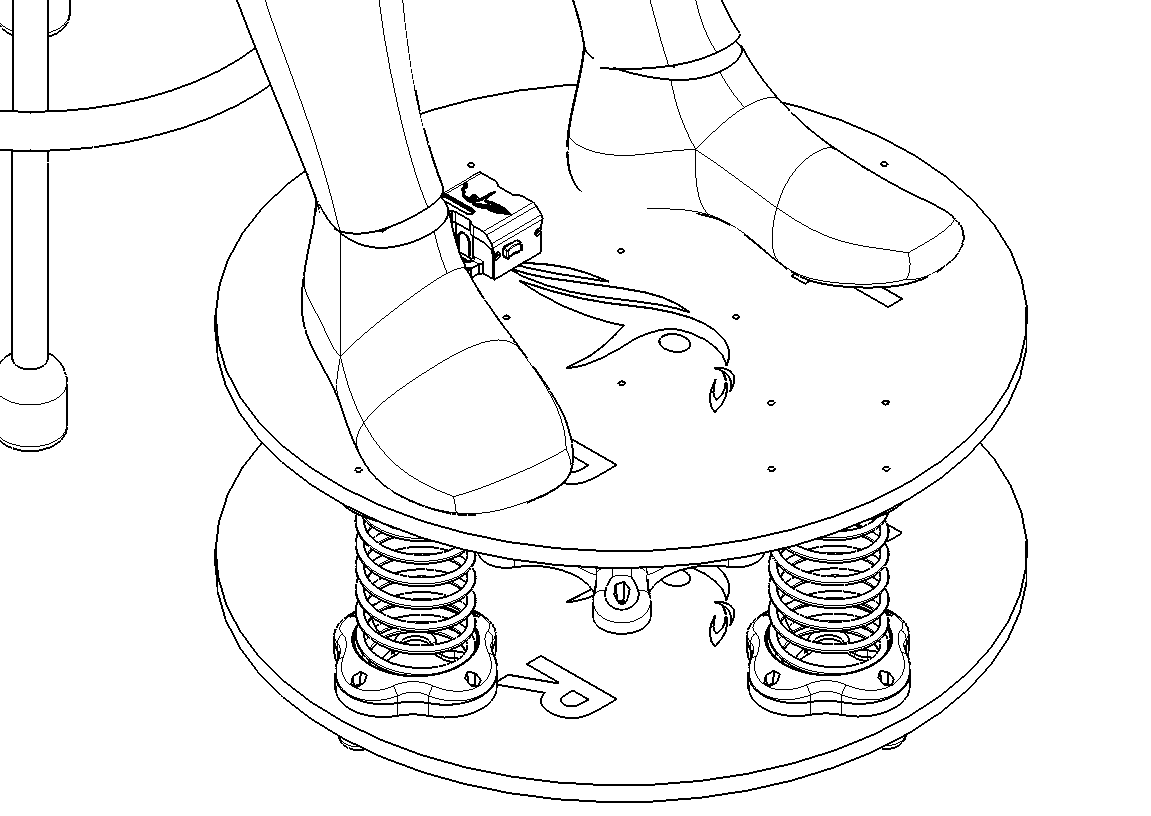
\includegraphics[width=0.6\textwidth,center]{Talaria_CloseUp.PNG}
\end{minipage}
\hfill
\begin{minipage}{0.65\textwidth}
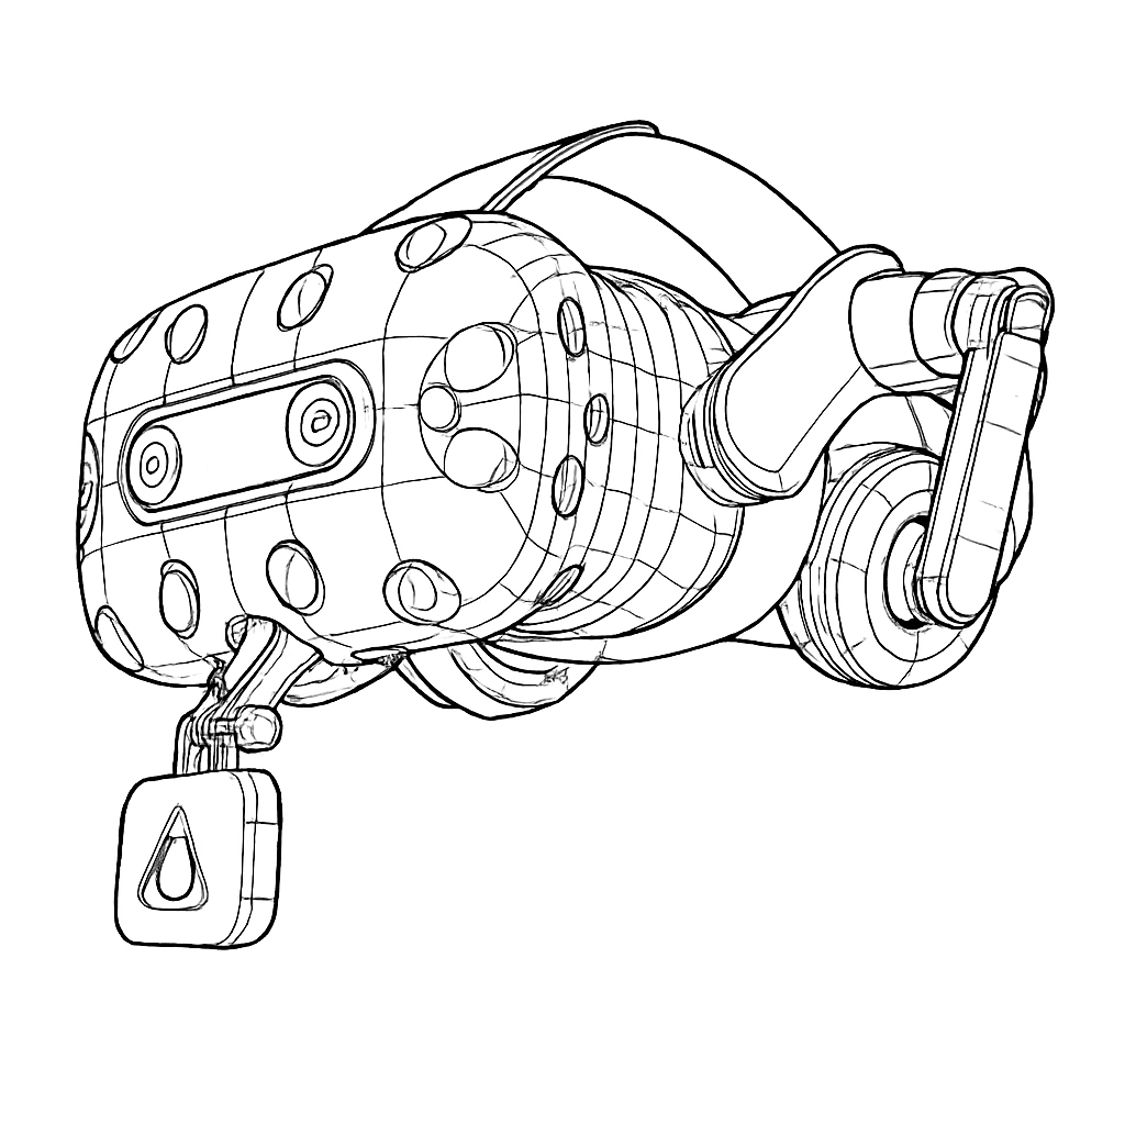
\includegraphics[width=0.5\textwidth,left]{HTC_Pro_Eye.png}
\end{minipage}
\end{figure}

\vspace{-2em}

\begin{itemize}
    \item Robot Humanoide:
    \begin{itemize}
    \item Plataforma robótica humanoide con arquitectura mecánica modular.
    \item Dos brazos robóticos (izquierdo y derecho) de 6 grados de libertad cada uno, con actuadores y reductores armónicos, capaces de manipular cargas de hasta 5 kg.
    \item Sujetadores adaptativos de tres dedos, dos falanges por dedo y un grado de libertad, optimizados para alto torque en espacio compacto.
    \item Torso con 2 grados de libertad, implementados mediante motores en configuración diferencial, que permiten inclinaciones laterales y frontales.
    \item Cabeza robótica equipada con cámaras estereoscópicas, micrófonos binaurales y proyección facial, que replica gestos del operador en tiempo real.
    \item Cuello articulado con 2 grados de libertad (pitch y yaw) para ampliar el campo visual.
    \item Base móvil diferencial con tracción trasera y sensores LiDAR para navegación asistida y prevención de colisiones.
    \end{itemize}
 \end{itemize}

\section{Caracterización del Sistema Prometheus 3.0}
\centering
\begin{tabular}{ccc}
\toprule
 & Valor & Unidad \\
\midrule
Peso & 105 & $kg$ \\
Dimensiones & 71*74*170 & $cm*cm*cm$ \\
Grados de Libertad & 20 & $GDL$ \\
Tiempo de Operación & 5 & $horas$ \\

\bottomrule
\end{tabular}

\raggedright

\subsection{Subsistemas del Humanoide}
\begin{center}
\begin{minipage}{0.4\textwidth}
\centering
\begin{tabular}{lcr}
\toprule
Núm & Subsistema \\
\midrule
1 & Cabeza (Rostro interactivo)\\
2 & Cuello (2 GDL)\\
3 & Torso  (2 GDL)\\
4 & Brazos (6 GDL por brazo) \\
5 & Grippers (1 GDL por gripper) \\
6 & Base móvil (2 GDL) \\
\bottomrule
\end{tabular}
\end{minipage}%
\begin{minipage}{0.6\textwidth}
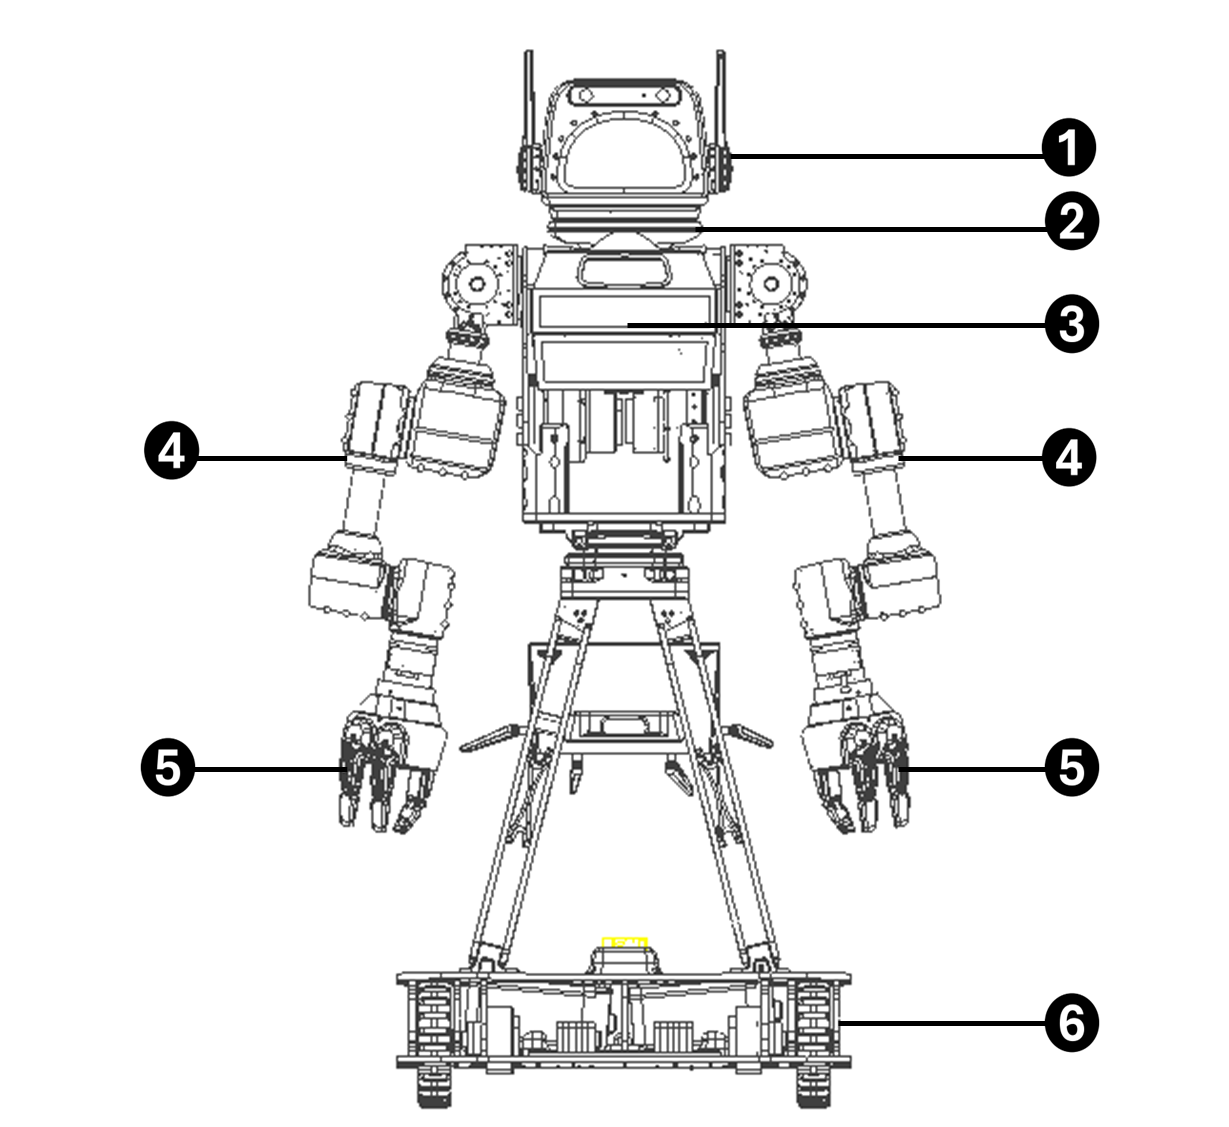
\includegraphics[width=0.6\textwidth,center]{PR3frontNum.png}
\end{minipage}
\end{center}

\subsection{Elementos de la Cabina de Operación}
\begin{center}
\begin{minipage}{0.4\textwidth}
\centering
\begin{tabular}{lcr}
\toprule
Núm & Elemento \\
\midrule
1 & Bases para el Headset\\
2 & Headset Vive Pro Eye\\
3 & Guantes Hápticos\\
4 & Cadena de Sensores Hermes \\
5 & Sistema de Dirección Plantar\\
\bottomrule
\end{tabular}
\end{minipage}%
\begin{minipage}{0.6\textwidth}
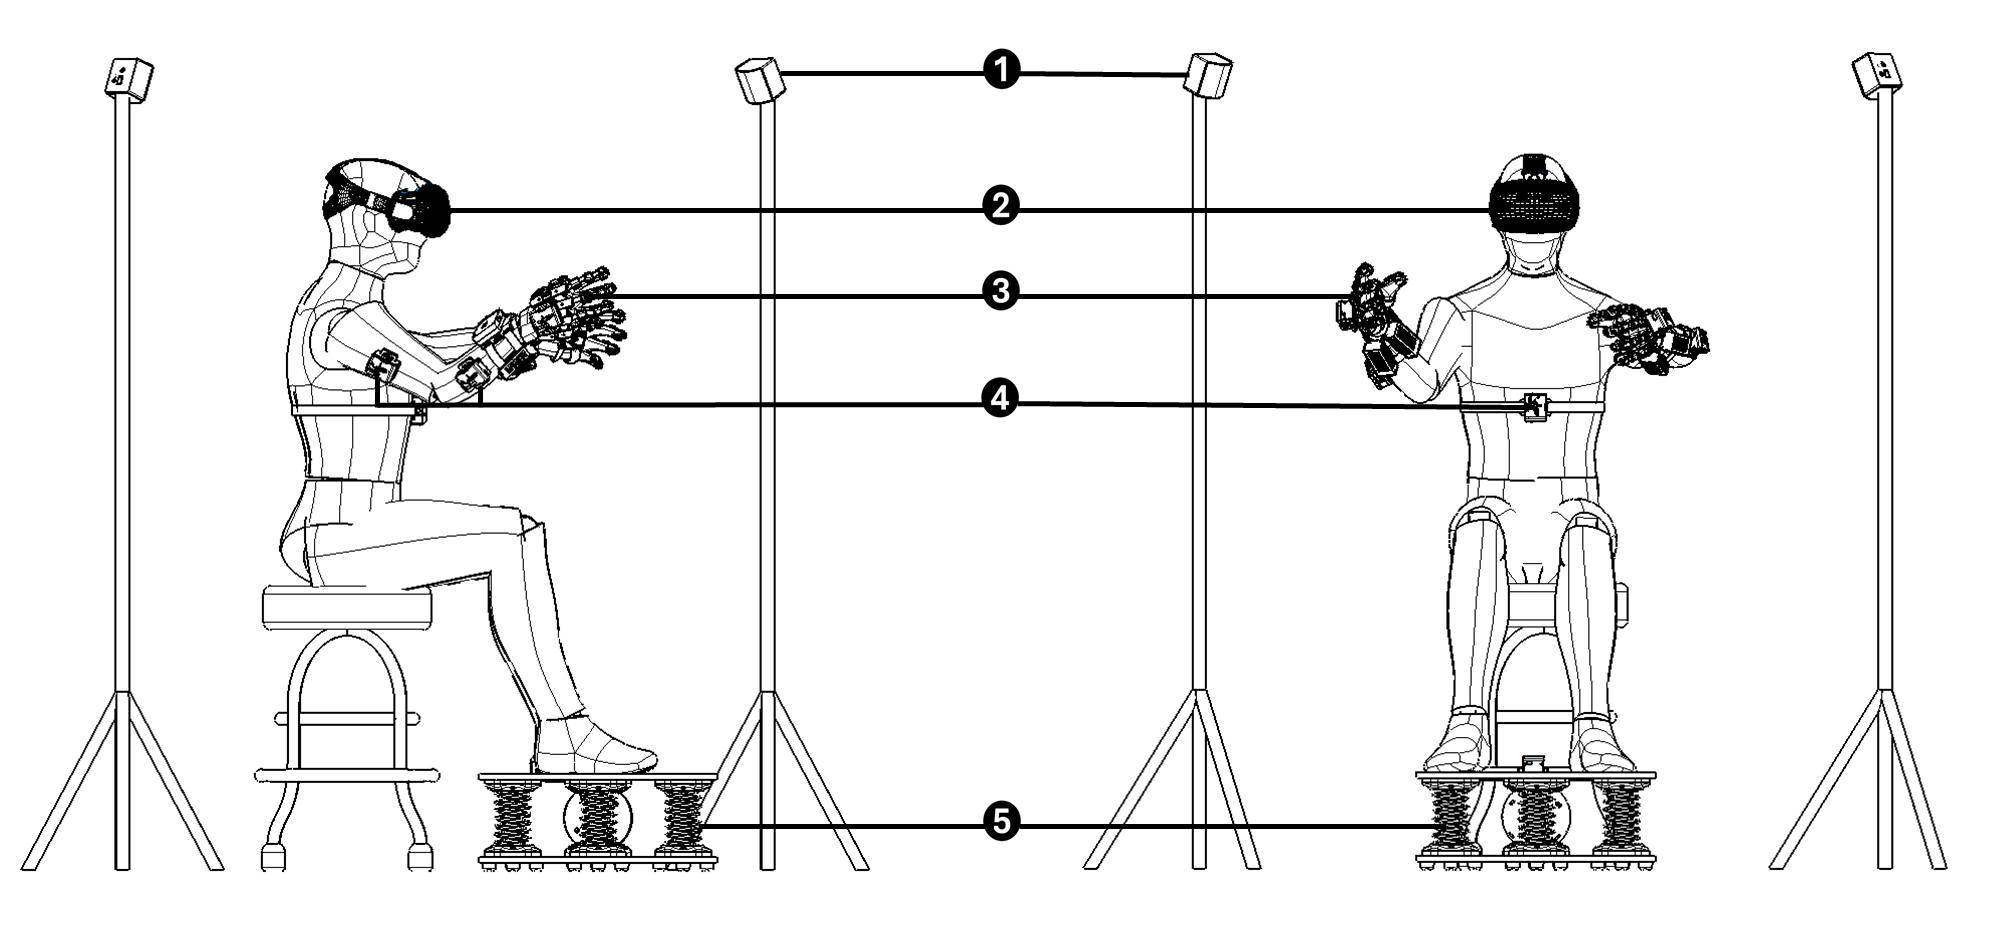
\includegraphics[width=\linewidth, left]{CabinaNumbered.png}
\end{minipage}
\end{center}

\subsection{Dimensiones Recomendadas para Teleoperación}
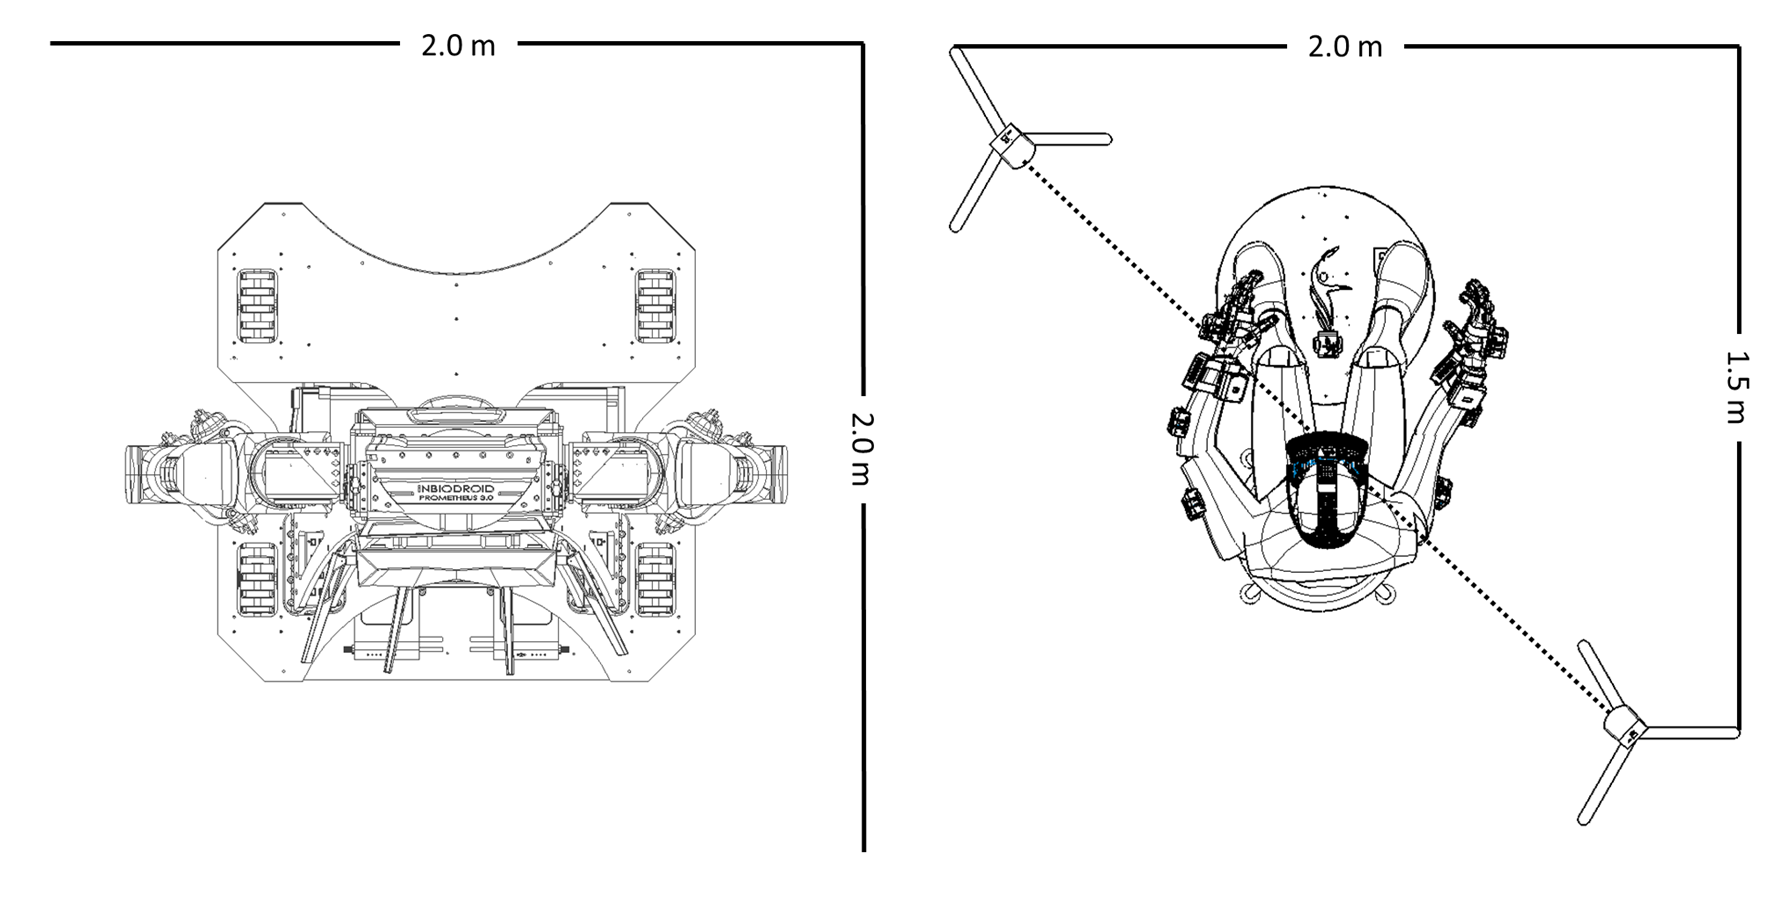
\includegraphics[width=0.6\textwidth, center]{Dimensions.png}

\section{Baterías}
\begin{itemize}
    \item El sistema robótico integra baterías LiPo modelos \textbf{TATTU Pro}, \textbf{Tattu Plus 6s} y \textbf{Tattu Plus 1.0}, seleccionadas por su compatibilidad con aplicaciones robóticas y su conjunto de funciones inteligentes.
    \item Estas baterías incorporan capacidades de monitoreo y gestión, incluyendo recolección y transmisión de datos, recordatorios de seguridad y carga, cálculo de energía, balanceo automático de celdas y alarmas ante condiciones anómalas.
\end{itemize}

\subsection{Ubicación de las Baterías}
\begin{center}
\begin{tabular}{lcr}
\toprule
Núm & Batería & Capacidad \\
\midrule
1 & Tattu Plus 1.0 & 22000mAh\\
2 & Tattu Pro & 22000mAh\\
3 & Tattu Plus 6s & 22000mAh \\
4 & Tattu Plus 6s & 22000mAh \\
\bottomrule
\end{tabular}

\vspace{2em}

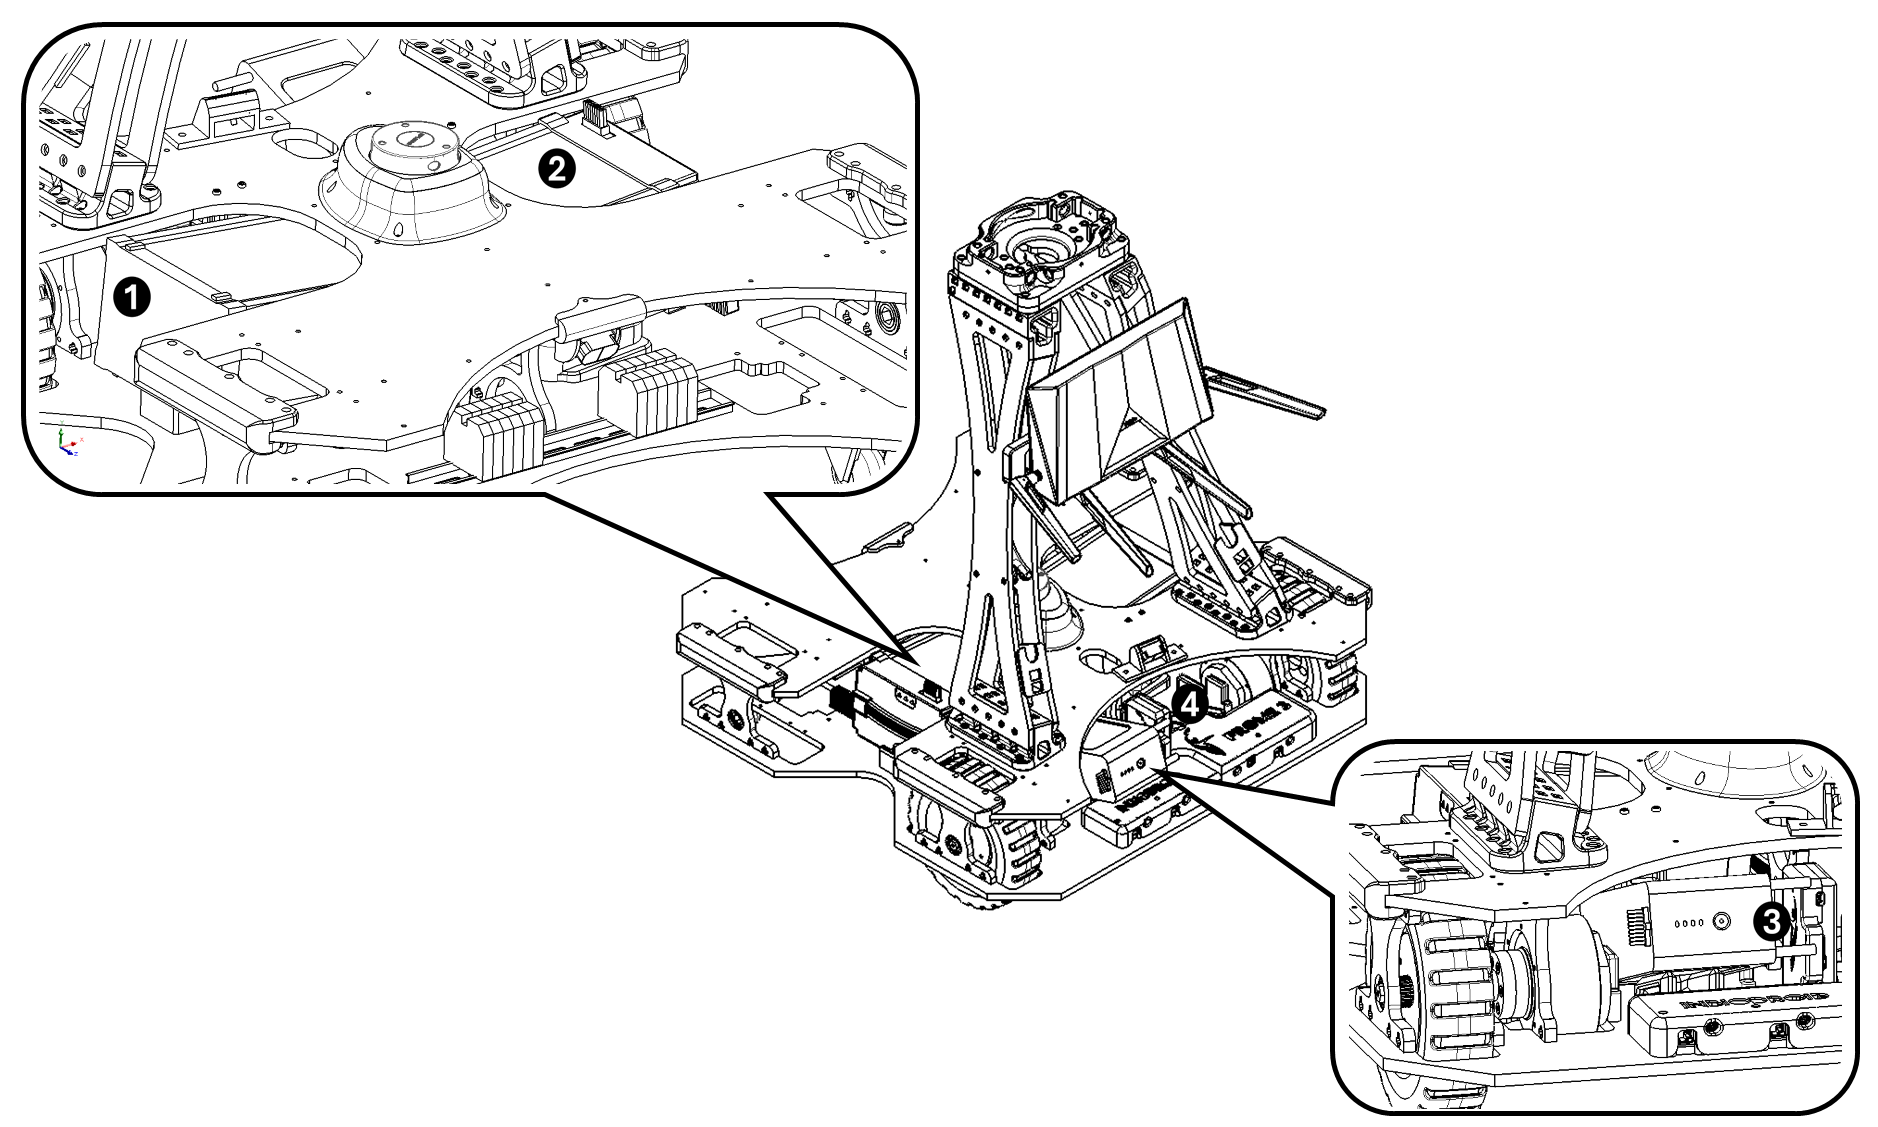
\includegraphics[width=\linewidth, left]{Batteries.png}
\end{center}

\subsection{Precauciones}
\begin{itemize}
    \item La batería de polímero de litio es un material activo y puede provocar incendios si no se utiliza correctamente.
    \item El uso inadecuado puede causar lesiones personales y daños materiales.
    \item La placa de protección de la batería no cuenta con función anti-chispa.
    \item Si se requiere esta función, utilice un conector con sistema anti-chispa.
    \item La batería no dispone de protección interna contra sobrecarga ni sobredescarga.
    \item Es obligatorio configurar correctamente los límites de voltaje de carga y descarga en el cargador o en el dispositivo.
    \item No cortocircuite el conector, ya que esto representa un riesgo grave de seguridad.
    \item Los cables de descarga deben estar correctamente soldados al conector.
    \item Una conexión deficiente puede causar pérdida de potencia y provocar fallos durante la operación.
    \item No tire de los cables de la batería en ninguna circunstancia.
\end{itemize}
\subsection{Uso}
\begin{itemize}
    \item Antes de utilizar la batería, verifique el nivel de carga y el estado de salud.
    \item Revise siempre el estado exterior de la batería.
    \item No la utilice si presenta:
    \begin{itemize}
        \item Daños físicos
        \item Inflado
        \item Fugas de electrolito
    \end{itemize}
    \item No permita que la batería ni el conector entren en contacto con metal o materiales de fibra de carbono, para evitar cortocircuitos.
    \item No cortocircuite ni invierta la polaridad (positivo y negativo).
    \item No tire de los cables de carga o descarga durante la manipulación.
    \item No desmonte, reensamble ni reorganice celdas de baterías.
    \item Estas prácticas son extremadamente peligrosas y pueden causar cortocircuitos e incendios.
    \item En ambientes de baja temperatura (por debajo de 5 °C):
        \begin{itemize}
        \item Precaliente la batería cargándola o descargándola con corriente baja hasta superar los 5 °C.
        \item La temperatura óptima de operación es 20 °C.
        \item No realice operaciones de alta carga con una batería fría.
        \item Permita que la batería alcance su temperatura normal antes de un uso intensivo.
    \end{itemize}
    \item No sobredescargue la batería.
    \item El voltaje por celda no debe ser inferior a 3.3 V, ya que la sobredescarga puede causar daños permanentes e inflado.
    \item No permita que el electrolito entre en contacto con los ojos o la piel.
    \item En caso de contacto, lave inmediatamente con agua y busque atención médica.
\end{itemize}
\subsection{Carga / Descarga}
\begin{itemize}
    \item Utilice únicamente cargadores inteligentes diseñados para baterías Li-Po / Li-ion.
    \item No utilice cargadores NiMH, NiCd, $LiFePO_\text{4}$ o plomo-ácido.
    \item Si el cargador admite varios tipos de batería, asegúrese de seleccionar correctamente el modo LiPo.
    \item La corriente de balanceo no debe superar 1 A.
    \item La corriente y el voltaje de carga deben ser inferiores a los valores máximos especificados por el fabricante.
    \item Se recomienda cargar y descargar la batería en un rango de temperatura de 10 °C a 45 °C (para operación general, se recomienda entre 0 °C y 40 °C).
    \item No cargue ni descargue la batería sin supervisión.
    \item Durante la carga:
        \begin{itemize}
            \item Utilice una superficie resistente al calor.
            \item Cargue en un área despejada y abierta, preferentemente sobre suelo de cemento.
            \item Se recomienda el uso de una bolsa ignífuga para baterías Li-Po.
            \item Mantenga la batería alejada de materiales inflamables o explosivos.
            \item Nunca cargue la batería instalada en el equipo ni dentro de un vehículo.
    \end{itemize}
    \item Nunca sobrecargue la batería.
    \item El voltaje máximo por celda no debe superar 4.25 V.
    \item Está prohibida la carga inversa.
\end{itemize}
\subsection{Almacenamiento}
\begin{itemize} 
    \item Evite el contacto con líquidos.
    \item No coloque la batería cerca de líquidos o agua, ni la almacene en ambientes húmedos.
    \item Manténgala alejada de fuentes de calor.
    \item No coloque la batería cerca de llamas abiertas, calentadores u otras fuentes de calor.
    \item Manténgala fuera del alcance de los niños.
    \item Condiciones de temperatura.
    \item Almacene la batería en un ambiente con temperatura controlada de aproximadamente 25 °C.
    \item Espacio de almacenamiento adecuado.
    \item Guarde la batería en un lugar despejado, asegurándose de que no esté comprimida ni aplastada.
    \item No apile baterías durante su almacenamiento.  
    \item Almacenamiento prolongado y mantenimiento periódico. Si la batería no se utiliza durante un periodo prolongado:
    \begin{itemize}
        \item Mantenga el voltaje por celda entre 3.8 y 3.9 V (nivel de almacenamiento).
        \item Revise la batería al menos cada 3 meses.
        \item Realice un ciclo de mantenimiento para preservar su vida útil:
        \begin{itemize}
            \item Cargue la batería a 0.2C hasta 4.2 V por celda,
            \item Déjela reposar 5 minutos,
            \item Descárguela a 0.2C hasta 3.46 V por celda,
            \item Déjela reposar 5 minutos,
            \item Vuelva a cargarla a 0.2C hasta 3.85–3.9 V por celda para su almacenamiento.
        \end{itemize}
    \end{itemize}
\end{itemize}
\end{document}
